
%\documentclass[11pts,a4paper,amsmath,amssymb,floatfix]{article}%{report}%{book}
\documentclass[12pts,a4paper,amsmath,amssymb,floatfix]{article}%{report}%{book}
\usepackage{graphicx,wrapfig}% Include figure files
%\usepackage{dcolumn,enumerate}% Align table columns on decimal point
\usepackage{enumerate,enumitem}% Align table columns on decimal point
\usepackage{bm,dpfloat}% bold math
\usepackage[pdftex,bookmarks,colorlinks=true,urlcolor=rltblue,citecolor=blue]{hyperref}
\usepackage{amsfonts,amsmath,amssymb,stmaryrd,indentfirst}
\usepackage{times,psfrag}
\usepackage{natbib}
\usepackage{color}
\usepackage{units}
\usepackage{rotating}
\usepackage{multirow}

\usepackage{pifont}
\usepackage{subfigure}
\usepackage{subeqnarray}
\usepackage{ifthen} 
  
\usepackage{supertabular} 
\usepackage{moreverb}
\usepackage{fancyvrb}
\usepackage{listings}  
\usepackage{palatino} 
%\usepackage{doi}
\usepackage{longtable} 
\usepackage{float}
\usepackage{perpage,comment}
\MakeSorted{figure}
%\usepackage{pdflscape}

\definecolor{rltblue}{rgb}{0,0,0.75}

 
%\usepackage{natbib}
\usepackage{fancyhdr} %%%%
\pagestyle{fancy}%%%%
% with this we ensure that the chapter and section
% headings are in lowercase
%%%%\renewcommand{\chaptermark}[1]{\markboth{#1}{}}
\renewcommand{\sectionmark}[1]{\markright{\thesection\ #1}}
\fancyhf{} %delete the current section for header and footer
\fancyhead[LE,RO]{\bfseries\thepage}
\fancyhead[LO]{\bfseries\rightmark}
\fancyhead[RE]{\bfseries\leftmark}
\renewcommand{\headrulewidth}{0.5pt}
% make space for the rule
\fancypagestyle{plain}{%
\fancyhead{} %get rid of the headers on plain pages
\renewcommand{\headrulewidth}{0pt} % and the line
}

\def\newblock{\hskip .11em plus .33em minus .07em}
\usepackage{color}

%\usepackage{makeidx}
%\makeindex

\setlength\textwidth      {16.cm}
\setlength\textheight     {22.6cm}
\setlength\oddsidemargin  {-0.3cm}
\setlength\evensidemargin {0.3cm}

\setlength\headheight{14.49998pt} 
\setlength\topmargin{0.0cm}
\setlength\headsep{1.cm}
\setlength\footskip{1.cm}
\setlength\parskip{0pt} 
\setlength\parindent{0pt} 

%%% 
%%% Headers and Footers
\lhead[] {\text{\small{EG3521 -- Engineering Thermodynamics}}} 
%\chead[] {\text{\small{Session 2012/13}}}  
\lfoot[]{Module 03}  
%\cfoot[\thepage]{\thepage}
\rfoot[\text{\small{\thepage}}]{\thepage}
\rhead[] {{\text{\small{Session 2013/14}}}}
\renewcommand{\headrulewidth}{0.8pt}
 
%%% 
%%% space between lines
%%%
\renewcommand{\baselinestretch}{1.5}

\newenvironment{VarDescription}[1]%
  {\begin{list}{}{\renewcommand{\makelabel}[1]{\textbf{##1:}\hfil}%
    \settowidth{\labelwidth}{\textbf{#1:}}%
    \setlength{\leftmargin}{\labelwidth}\addtolength{\leftmargin}{\labelsep}}}%
  {\end{list}}

%%%%%%%%%%%%%%%%%%%%%%%%%%%%%%%%%%%%%%%%%%%
%%%%%%                              %%%%%%%
%%%%%%      NOTATION SECTION        %%%%%%%
%%%%%%                              %%%%%%%
%%%%%%%%%%%%%%%%%%%%%%%%%%%%%%%%%%%%%%%%%%%

% Text abbreviations.
\newcommand{\ie}{{\em{i.e., }}}
\newcommand{\eg}{{\em{e.g., }}}
\newcommand{\cf}{{\em{cf., }}}
\newcommand{\wrt}{with respect to}
\newcommand{\lhs}{left hand side}
\newcommand{\rhs}{right hand side}
% Commands definining mathematical notation.

% This is for quantities which are physically vectors.
\renewcommand{\vec}[1]{{\mbox{\boldmath$#1$}}}
% Physical rank 2 tensors
\newcommand{\tensor}[1]{\overline{\overline{#1}}}
% This is for vectors formed of the value of a quantity at each node.
\newcommand{\dvec}[1]{\underline{#1}}
% This is for matrices in the discrete system.
\newcommand{\mat}[1]{\mathrm{#1}}


\DeclareMathOperator{\sgn}{sgn}
\newtheorem{thm}{Theorem}[section]
\newtheorem{lemma}[thm]{Lemma}

%\newcommand\qed{\hfill\mbox{$\Box$}}
\newcommand{\re}{{\mathrm{I}\hspace{-0.2em}\mathrm{R}}}
\newcommand{\inner}[2]{\langle#1,#2\rangle}
\renewcommand\leq{\leqslant}
\renewcommand\geq{\geqslant}
\renewcommand\le{\leqslant}
\renewcommand\ge{\geqslant}
\renewcommand\epsilon{\varepsilon}
\newcommand\eps{\varepsilon}
\renewcommand\phi{\varphi}
\newcommand{\bmF}{\vec{F}}
\newcommand{\bmphi}{\vec{\phi}}
\newcommand{\bmn}{\vec{n}}
\newcommand{\bmns}{{\textrm{\scriptsize{\boldmath $n$}}}}
\newcommand{\bmi}{\vec{i}}
\newcommand{\bmj}{\vec{j}}
\newcommand{\bmk}{\vec{k}}
\newcommand{\bmx}{\vec{x}}
\newcommand{\bmu}{\vec{u}}
\newcommand{\bmv}{\vec{v}}
\newcommand{\bmr}{\vec{r}}
\newcommand{\bma}{\vec{a}}
\newcommand{\bmg}{\vec{g}}
\newcommand{\bmU}{\vec{U}}
\newcommand{\bmI}{\vec{I}}
\newcommand{\bmq}{\vec{q}}
\newcommand{\bmT}{\vec{T}}
\newcommand{\bmM}{\vec{M}}
\newcommand{\bmtau}{\vec{\tau}}
\newcommand{\bmOmega}{\vec{\Omega}}
\newcommand{\pp}{\partial}
\newcommand{\kaptens}{\tensor{\kappa}}
\newcommand{\tautens}{\tensor{\tau}}
\newcommand{\sigtens}{\tensor{\sigma}}
\newcommand{\etens}{\tensor{\dot\epsilon}}
\newcommand{\ktens}{\tensor{k}}
\newcommand{\half}{{\textstyle \frac{1}{2}}}
\newcommand{\tote}{E}
\newcommand{\inte}{e}
\newcommand{\strt}{\dot\epsilon}
\newcommand{\modu}{|\bmu|}
% Derivatives
\renewcommand{\d}{\mathrm{d}}
\newcommand{\D}{\mathrm{D}}
\newcommand{\ddx}[2][x]{\frac{\d#2}{\d#1}}
\newcommand{\ddxx}[2][x]{\frac{\d^2#2}{\d#1^2}}
\newcommand{\ddt}[2][t]{\frac{\d#2}{\d#1}}
\newcommand{\ddtt}[2][t]{\frac{\d^2#2}{\d#1^2}}
\newcommand{\ppx}[2][x]{\frac{\partial#2}{\partial#1}}
\newcommand{\ppxx}[2][x]{\frac{\partial^2#2}{\partial#1^2}}
\newcommand{\ppt}[2][t]{\frac{\partial#2}{\partial#1}}
\newcommand{\pptt}[2][t]{\frac{\partial^2#2}{\partial#1^2}}
\newcommand{\DDx}[2][x]{\frac{\D#2}{\D#1}}
\newcommand{\DDxx}[2][x]{\frac{\D^2#2}{\D#1^2}}
\newcommand{\DDt}[2][t]{\frac{\D#2}{\D#1}}
\newcommand{\DDtt}[2][t]{\frac{\D^2#2}{\D#1^2}}
% Norms
\newcommand{\Ltwo}{\ensuremath{L_2} }
% Basis functions
\newcommand{\Qone}{\ensuremath{Q_1} }
\newcommand{\Qtwo}{\ensuremath{Q_2} }
\newcommand{\Qthree}{\ensuremath{Q_3} }
\newcommand{\QN}{\ensuremath{Q_N} }
\newcommand{\Pzero}{\ensuremath{P_0} }
\newcommand{\Pone}{\ensuremath{P_1} }
\newcommand{\Ptwo}{\ensuremath{P_2} }
\newcommand{\Pthree}{\ensuremath{P_3} }
\newcommand{\PN}{\ensuremath{P_N} }
\newcommand{\Poo}{\ensuremath{P_1P_1} }
\newcommand{\PoDGPt}{\ensuremath{P_{-1}P_2} }

\newcommand{\metric}{\tensor{M}}
\newcommand{\configureflag}[1]{\texttt{#1}}

% Units
\newcommand{\m}[1][]{\unit[#1]{m}}
\newcommand{\km}[1][]{\unit[#1]{km}}
\newcommand{\s}[1][]{\unit[#1]{s}}
\newcommand{\invs}[1][]{\unit[#1]{s}\ensuremath{^{-1}}}
\newcommand{\ms}[1][]{\unit[#1]{m\ensuremath{\,}s\ensuremath{^{-1}}}}
\newcommand{\mss}[1][]{\unit[#1]{m\ensuremath{\,}s\ensuremath{^{-2}}}}
\newcommand{\K}[1][]{\unit[#1]{K}}
\newcommand{\PSU}[1][]{\unit[#1]{PSU}}
\newcommand{\Pa}[1][]{\unit[#1]{Pa}}
\newcommand{\kg}[1][]{\unit[#1]{kg}}
\newcommand{\rads}[1][]{\unit[#1]{rad\ensuremath{\,}s\ensuremath{^{-1}}}}
\newcommand{\kgmm}[1][]{\unit[#1]{kg\ensuremath{\,}m\ensuremath{^{-2}}}}
\newcommand{\kgmmm}[1][]{\unit[#1]{kg\ensuremath{\,}m\ensuremath{^{-3}}}}
\newcommand{\Nmm}[1][]{\unit[#1]{N\ensuremath{\,}m\ensuremath{^{-2}}}}

% Dimensionless numbers
\newcommand{\dimensionless}[1]{\mathrm{#1}}
\renewcommand{\Re}{\dimensionless{Re}}
\newcommand{\Ro}{\dimensionless{Ro}}
\newcommand{\Fr}{\dimensionless{Fr}}
\newcommand{\Bu}{\dimensionless{Bu}}
\newcommand{\Ri}{\dimensionless{Ri}}
\renewcommand{\Pr}{\dimensionless{Pr}}
\newcommand{\Pe}{\dimensionless{Pe}}
\newcommand{\Ek}{\dimensionless{Ek}}
\newcommand{\Gr}{\dimensionless{Gr}}
\newcommand{\Ra}{\dimensionless{Ra}}
\newcommand{\Sh}{\dimensionless{Sh}}
\newcommand{\Sc}{\dimensionless{Sc}}


% Journals
\newcommand{\IJHMT}{{\it International Journal of Heat and Mass Transfer}}
\newcommand{\NED}{{\it Nuclear Engineering and Design}}
\newcommand{\ICHMT}{{\it International Communications in Heat and Mass Transfer}}
\newcommand{\NET}{{\it Nuclear Engineering and Technology}}
\newcommand{\HT}{{\it Heat Transfer}}   
\newcommand{\IJHT}{{\it International Journal for Heat Transfer}}

\newcommand{\frc}{\displaystyle\frac}

\newlist{ExList}{enumerate}{1}
\setlist[ExList,1]{label={\bf Example 1.} {\bf \arabic*}}

\newlist{ProbList}{enumerate}{1}
\setlist[ProbList,1]{label={\bf Problem 1.} {\bf \arabic*}}

%%%%%%%%%%%%%%%%%%%%%%%%%%%%%%%%%%%%%%%%%%%
%%%%%%                              %%%%%%%
%%%%%% END OF THE NOTATION SECTION  %%%%%%%
%%%%%%                              %%%%%%%
%%%%%%%%%%%%%%%%%%%%%%%%%%%%%%%%%%%%%%%%%%%


% Cause numbering of subsubsections. 
%\setcounter{secnumdepth}{8}
%\setcounter{tocdepth}{8}

\setcounter{secnumdepth}{4}%
\setcounter{tocdepth}{4}%


\DeclareMathAlphabet{\mathpzc}{OT1}{pzc}{m}{it}

\begin{document}


%%%
%%%  First Page
%%%
\begin{comment}
\begin{titlepage}

\begin{center}
\bigskip
 
\vspace{4.cm}
\begin{center}
\resizebox{80mm}{!}{
\includegraphics[clip=true]{../FigBanner/UoALarge}}
\end{center}

\vspace{3.5cm}
\bigskip

{\bf {\huge  EG3521: Engineering Thermodynamics}} \\

\bigskip
{\bf {\huge Module 03: Refrigeration and Liquefaction}}\\
{\bf {\Large Examples and Problems}}
\bigskip
\vspace{5.cm}

{\bf {\Large Dr Jeff Gomes}}
\bigskip

{\bf{\Large  School of Engineering}}\\
\vspace{3cm}    

\bigskip 

{\bf {\large \today}}
\end{center}
 

\end{titlepage}
\end{comment}

\setcounter{page}{1}

\vfill

\begin{description}
\item[Problem] A power system was designed to operate with two turbines and a regenerator as shown in Figure~\ref{Ex1}. The system generates a net power of
\begin{displaymath}
\Phi = \sum W_{\text{Turbines}} -\sum W_{\text{Pumps}}
\end{displaymath}
and is coupled to a reversed-Rankine cycle to provide heating to a controlled environment. The heat extracted from the condenser (5-6) is fully transferred to the refrigerant fluid (13-10), i.e.,
\begin{displaymath}
Q_{\text{Condenser}} = \dot{m}_{w}^{5-6}\left(H_{5}-H_{6}\right)=\dot{m}_{R}\left(H_{10}-H_{13}\right)
\end{displaymath} 
where $\dot{m}_{w}^{5-6}$ and $\dot{m}_{R}\;\left(=2\;kg/s\right)$ are the mass flow rates of water/steam leaving the Turbine LP and the refrigerant fluid R134a. To solve this problem, you should assume that the saturated liquid streams are incompressible, and therefore $dH = VdP$ (where H, V and P are enthalpy, volume and pressure, respectively). The efficiencies associated with the HP and LP turbines and pumps 1 (P1) and 2 (P2) are 98.5, 99, 65 and 73$\%$, respectively. Assume that the mass flow rate of water/steam leaving boiler (stream 1) is 1 kg/s
\begin{enumerate}%[(1)] 
\item Calculate (A-W) and (i-ix) from the Table~\ref{Ex:Tab} {\bf [66 Marks]};
\item Calculate the heat suplied by the boiler {\bf [17 Marks]};
\item Calculate the thermal efficiency in the power cycle {\bf [17 Marks]}.
\end{enumerate}
\end{description}



\begin{table}[h]
\begin{center}
\begin{tabular}{ || c || c | c | c | c | c || c ||}
\hline\hline
{\bf Flow}& {\bf Pressure}  &  {\bf Temperature}   &  {\bf Enthalpy}  & {\bf Entropy}     & {\bf State}  & {\bf Quality of} \\
          & {\bf (bar)}     & {\bf ($^{\text{o}}$C)} &  {\bf (kJ/kg)}   &  {\bf (kJ/kg.K)}  &              & {\bf steam}      \\
\hline\hline
{\bf 1}   &   210.0         &      660         &      (A)          &      (B)             & (C)          &  --              \\
{\bf 2}   &   7.4           &       --         &      (D)          &      (E)             & wet vapour   &  (F)             \\
{\bf 3}   &   7.4           &      400         &      (G)          &      (H)             & (I)          &  --              \\
{\bf 4}   &   7.4           &      600         &      (J)          &      (K)             & (L)          &  --              \\ 
{\bf 5}   &   0.08          &      --          &      (M)          &      (N)             & (O)          &  (P)             \\ 
{\bf 6}   &   0.08          &      --          &      (Q)          &      (R)             & (S)          &  --              \\
{\bf 7}   &   7.4           &      --          &      (T)          &      --              & --           &   --             \\              
{\bf 8}   &   --            &      --          &      (U)          &      (V)             & --           & --               \\             
{\bf 9}   &   (W)           &      --          &      (Y)          &      --              & --           & --               \\
\hline \hline
{\bf 10}  &   (i)           &      --          &      (ii)         &      --             &  (iii)        &  --              \\
{\bf 11}  &  --             &      --          &      --           &      --             &   --          &   --             \\ 
{\bf 12}  &  6.3            &     5.6          &      (iv)         &      (v)            &  (vi)         &   --             \\
{\bf 13}  &  3.2            &     --           &     (vii)         &      (viii)         &   --         &    (ix)            \\ 
\hline\hline
\end{tabular}
\end{center}
\caption{Information on the steam-power and refrigeration cycles.}\label{Ex:Tab}
\end{table}


\begin{figure}[h]
\begin{center}
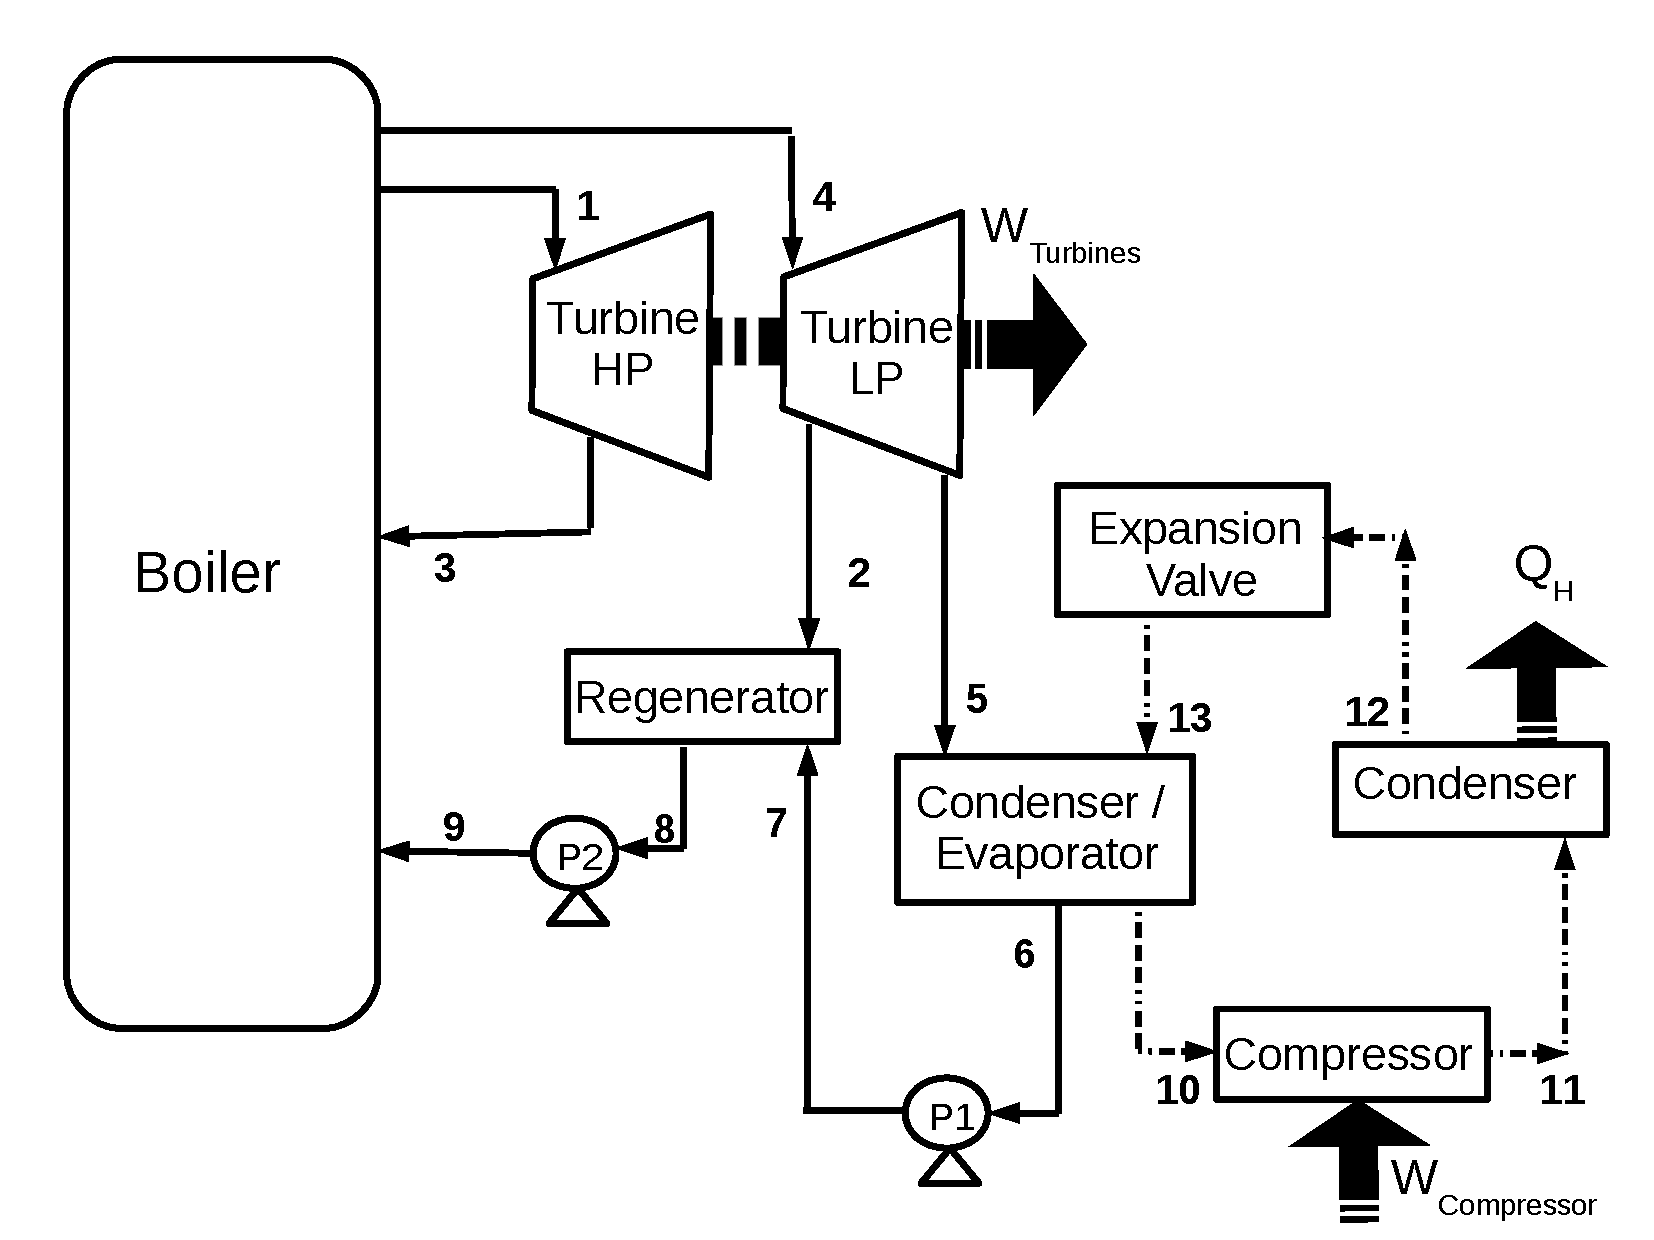
\includegraphics[width=19.0cm,height=15.0cm,angle=-90.]{./Pics/ExtraQuestionPic}
\end{center}
\caption{Regenerative Reheat Rankine (full line) and Reverse Rankine (dotline) cycles.}\label{Ex1}
\end{figure}

\end{document}
